\documentclass{article}
\usepackage[utf8]{inputenc}
\usepackage[T1]{fontenc}
\usepackage{graphicx}
\usepackage{hyperref}
\usepackage{geometry}
\geometry{margin=1in}

\title{HELOTS}
\date{Encyclopaedia Britannica (1771)}

\begin{document}
\maketitle

\section*{Historical source}
\textbf{Entry ID:} \texttt{entry-helots-1017} \\
\textbf{Volume ID:} 144850367 \\
\textbf{Character Count:} 358

\subsection*{Extracted Text}
HELOTS, in Grecian antiquity, the inhabitants of Helon, a town of Lacom, conquer by the Spartan; who made them all prisoners of var, and reduced them into the condition of flares.

The femme of Sparta were forbidden the excerite of any mean on mechanical employment, and therefore the whole care of fupplying the city with necefairs devoted upon the filters.



\section*{Source record}
\begin{itemize}
\item \textbf{Dataset:} \texttt{NationalLibraryOfScotland/encyclopaedia\_britannica\_illustrated}
\item \textbf{Dataset Revision:} \texttt{309f765b1ecc83e0a7f7762e44b4a927a7555443}
\item \textbf{Page ID:} \texttt{britannica:309f765b1ecc83e0a7f7762e44b4a927a7555443:train:1017} \\
  \textbf{Filename:} \texttt{page-1017-5395deb0e141.jpg} \\
  \textbf{Row Index:} 1017 \\
  \textbf{SHA256:} \texttt{5395deb0e1413694...}
\end{itemize}

\begin{figure}[h]
\centering
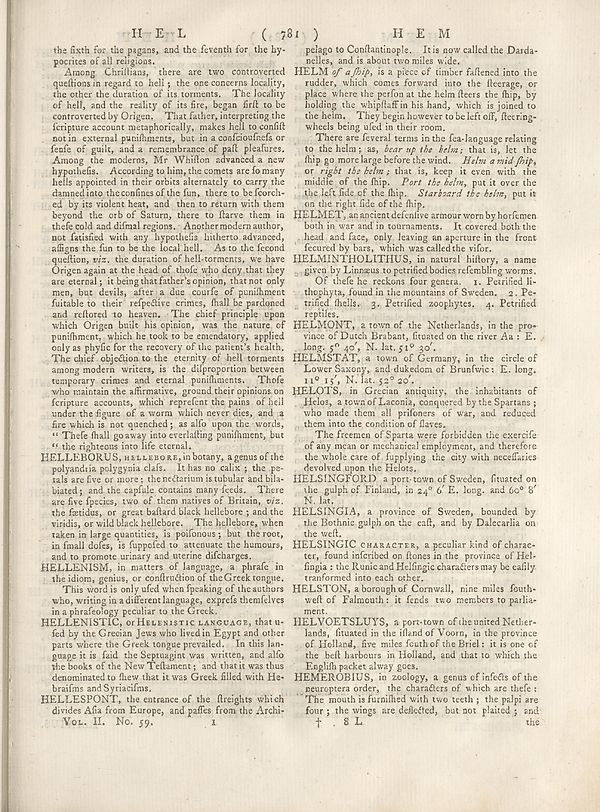
\includegraphics[width=0.85\textwidth]{../scans/page-1017-5395deb0e141.jpg}
\caption*{Source scan: \texttt{page-1017-5395deb0e141.jpg}}
\end{figure}

\end{document}
